\documentclass[11pt,a4paper]{article}

% Compilar com lualatex (UTF-8 nativo). Ex.:
%   lualatex -interaction=nonstopmode relatorio_fase2.tex   (2x)
\usepackage{fontspec}
% Fonte Helvetica (TeX Gyre Heros), igual ao relatorio da Fase 1
\setmainfont{TeX Gyre Heros}
\setsansfont{TeX Gyre Heros}
\usepackage[brazil]{babel}
\usepackage[a4paper,margin=2.5cm]{geometry}
\usepackage{graphicx}
\usepackage[table]{xcolor}
\usepackage{listings}
\usepackage{booktabs}
\usepackage{array}
\usepackage{tikz}
\usetikzlibrary{positioning,arrows.meta,calc,fit}
\usepackage{fancyhdr}
\usepackage[hidelinks]{hyperref}
\usepackage{enumitem}

% ----- Cores e estilo de código -----
\definecolor{corFundo}{RGB}{248,248,248}
\definecolor{corComent}{RGB}{106,115,125}
\definecolor{corKw}{RGB}{167,29,93}
\definecolor{corStr}{RGB}{3,47,98}
\definecolor{corMoldura}{RGB}{210,210,210}
\definecolor{corDestaque}{RGB}{255,245,200}

\lstset{
  basicstyle=\ttfamily\footnotesize,
  backgroundcolor=\color{corFundo},
  frame=single,
  rulecolor=\color{corMoldura},
  breaklines=true,
  breakatwhitespace=false,
  columns=fullflexible,
  keepspaces=true,
  showstringspaces=false,
  extendedchars=true,
  commentstyle=\color{corComent}\itshape,
  keywordstyle=\color{corKw}\bfseries,
  stringstyle=\color{corStr},
  numbers=left,
  numberstyle=\tiny\color{corComent},
  numbersep=8pt,
  tabsize=4,
  captionpos=b,
  xleftmargin=16pt,
}

% Estilo para saídas de terminal / capturas (sem realce de sintaxe)
\lstdefinestyle{saida}{
  language=,
  keywordstyle=\color{black},
  commentstyle=\color{black},
  stringstyle=\color{black},
  numbers=none,
  basicstyle=\ttfamily\scriptsize,
}

\pagestyle{fancy}
\fancyhf{}
\lhead{\small Laboratório de Redes — Fase 2}
\rhead{\small Interceptação Ativa (MITM)}
\cfoot{\thepage}
\renewcommand{\headrulewidth}{0.4pt}

\setlength{\parskip}{0.5em}
\setlength{\parindent}{0pt}

% ---------------------------------------------------------------------------
\begin{document}

% =============================== CAPA ===============================
\begin{titlepage}
\centering
\vspace*{1.5cm}
{\large Pontifícia Universidade Católica do Rio Grande do Sul}\\[0.2cm]
{\large Escola Politécnica}\\[0.2cm]
{\large Laboratório de Redes de Computadores}\\[2.5cm]

\rule{\linewidth}{0.5mm}\\[0.5cm]
{\huge \bfseries Interceptação e Defesa de um\\ Protocolo de Aplicação}\\[0.4cm]
{\Large Fase 2 — Interceptação Ativa (Man-in-the-Middle)}\\[0.3cm]
{\large Proxy MITM concorrente: leitura e modificação de mensagens}\\
\rule{\linewidth}{0.5mm}\\[1.5cm]

{\large\bfseries Grupo}\\[0.3cm]
{\large
Gabriel Dienstmann Sieczkowski\\
Lorenzo Hubner Panato\\
Luis Felipe Kvieczinski\\
}
\vfill
{\large Entrega 2 — Demonstração da quebra de integridade e autenticação}\\[0.3cm]
{\large Outubro de 2026}
\end{titlepage}

\tableofcontents
\newpage

% =============================== 1. OBJETIVO ===============================
\section{Objetivo e escopo}

Este relatório documenta a \textbf{Fase 2} do trabalho, cuja meta é demonstrar a
\textbf{quebra de integridade e de autenticação} de um protocolo de aplicação
sem proteção. Enquanto a Fase 1 mostrou a escuta \emph{passiva} (quebra de
confidencialidade), a Fase 2 introduz um atacante \textbf{ativo}: um
\textbf{proxy man-in-the-middle (MITM)} posicionado entre o cliente e o
servidor, capaz de \textbf{ler e alterar} as mensagens em trânsito e de
\textbf{atender múltiplas sessões simultâneas}.

O serviço-alvo da Fase 1 (par cliente/servidor com autenticação em texto claro)
é \textbf{reutilizado sem alteração}. O único componente novo é o
\texttt{proxy\_mitm.py}. O desvio do tráfego é feito \textbf{por configuração},
apontando o cliente ao proxy — exatamente como pede o enunciado.

\paragraph{Escopo e ética.} O proxy é uma \textbf{prova de conceito} de uso
\textbf{exclusivo} em laboratório \textbf{isolado} (VMs do próprio grupo). Ele
explora a ausência de integridade/autenticação do protocolo para fundamentar a
defesa da Fase 3 (TLS + certificado + senhas com \textit{hash}).

\paragraph{Decisões de projeto.}
\begin{itemize}[nosep]
  \item \textbf{Redirecionamento:} por configuração do cliente
        (\texttt{cliente.py -{}-host <proxy>}); \textbf{sem} ARP spoofing nem
        proxy transparente.
  \item \textbf{Linguagem:} Python 3, usando \textbf{sockets diretamente}, sem
        frameworks que escondam o socket.
  \item \textbf{Concorrência:} \textit{threads} da biblioteca padrão — uma
        \textit{thread} por sentido de cada sessão.
\end{itemize}

% =============================== 2. TOPOLOGIA ===============================
\section{Topologia de redirecionamento}

O teste é feito em uma \textbf{rede interna isolada}. A antiga VM-observador da
Fase 1 passa a ser a \textbf{VM-atacante}, rodando o proxy. O cliente é
reconfigurado para conectar ao proxy, que encaminha para o servidor real.

\begin{figure}[h]
\centering
\begin{tikzpicture}[
  vm/.style={draw, rounded corners, align=center, minimum width=3.0cm,
             minimum height=1.4cm, fill=blue!5, thick},
  atk/.style={draw, rounded corners, align=center, minimum width=3.2cm,
              minimum height=1.4cm, fill=red!5, thick},
  font=\small
]
  \node[vm]  (cli) {\textbf{VM-cliente}\\\texttt{cliente.py}\\\texttt{10.0.0.10}};
  \node[atk,right=2.6cm of cli] (atk) {\textbf{VM-atacante}\\\texttt{proxy\_mitm.py}\\\texttt{10.0.0.30}};
  \node[vm,right=2.6cm of atk] (srv) {\textbf{VM-servidor}\\\texttt{servidor.py}\\\texttt{10.0.0.20}};

  \draw[-{Latex[length=3mm]}, thick]
     (cli) -- node[above,align=center]{\footnotesize TCP 5050} (atk);
  \draw[-{Latex[length=3mm]}, thick]
     (atk) -- node[above,align=center]{\footnotesize TCP 5050} (srv);

  \node[font=\scriptsize, below=3pt of cli] (lcli) {\texttt{-{}-host 10.0.0.30}};
  \node[font=\scriptsize, below=3pt of atk] (latk) {lê / altera};
  \node[font=\scriptsize, below=3pt of srv] (lsrv) {\textit{(inalterado)}};

  \node[draw, dotted, inner sep=0.45cm, fit=(cli)(srv)(lcli)(lsrv),
        label={[font=\footnotesize\itshape]below:Rede interna isolada (10.0.0.0/24) — sem Internet}] {};
\end{tikzpicture}
\caption{Topologia de redirecionamento: o cliente é apontado ao proxy
(\texttt{10.0.0.30}), que repassa ao servidor real (\texttt{10.0.0.20:5050}) e
pode ler/alterar cada mensagem nos dois sentidos.}
\label{fig:topologia}
\end{figure}

Diferente da Fase 1, o atacante \textbf{participa} da conexão: ele termina a
conexão TCP do cliente e abre uma segunda conexão ao servidor. Por isso
\textbf{não} é necessário modo promíscuo nem \textit{hub} — basta que o cliente
esteja configurado para falar com o proxy.

% =============================== 3. ARQUITETURA ===============================
\section{Arquitetura do proxy}

Para cada cliente aceito, o proxy abre a conexão ao servidor real e sobe
\textbf{duas threads de relay}, uma por sentido. Cada thread lê de um lado e
escreve no outro, processando o fluxo \textbf{linha a linha} (o protocolo é
textual, terminado em \texttt{\textbackslash n}) para poder inspecionar e, se
configurado, \textbf{adulterar} cada mensagem antes de repassá-la.

\begin{lstlisting}[language=Python,caption={Núcleo do relay de um sentido, com ponto de adulteração (trecho de \texttt{proxy\_mitm.py}).}]
while True:
    dados = origem.recv(BUFFER)
    if not dados:
        break  # a outra ponta fechou a conexao
    buffer += dados
    saida = b""
    while b"\n" in buffer:
        linha_bytes, buffer = buffer.split(b"\n", 1)
        original = linha_bytes.decode(ENCODING, errors="replace")
        modificada = adulterar(sessao, original)   # <-- le e pode alterar
        saida += (modificada + "\n").encode(ENCODING)
    if saida:
        destino.sendall(saida)
\end{lstlisting}

O bloco \texttt{adulterar} aplica as regras escolhidas por \textit{flag}
(Seção~\ref{sec:demo}); qualquer linha fora do padrão esperado passa
\textbf{inalterada}, o que também garante a robustez diante de mensagens
malformadas.

% =============================== 4. CONCORRÊNCIA ===============================
\section{Modelo de concorrência e regiões críticas}

O proxy usa uma \textbf{thread por sentido} de cada sessão, mais a thread
principal de \texttt{accept()}. Para \textbf{N} sessões simultâneas há
\textbf{2N + 1} threads. As sessões \textbf{não compartilham estado de protocolo
entre si}, de modo que a maior parte do código dispensa travas. Há exatamente
três regiões críticas, resumidas na Tabela~\ref{tab:regioes}; o documento
\texttt{fase2/concorrencia.md} traz a discussão completa (entrega 3).

\begin{table}[h]
\centering\small
\begin{tabular}{@{}lp{4.1cm}p{5.6cm}@{}}
\toprule
\textbf{\#} & \textbf{Recurso compartilhado} & \textbf{Proteção} \\
\midrule
1 & Saída padrão (log do proxy) & \texttt{\_lock\_log} global: a função \texttt{log()} imprime cada linha dentro do lock \\
2 & Contador de IDs de sessão & \texttt{itertools.count} (atômico sob o GIL); impresso via \texttt{log()} \\
3 & Campo \texttt{usuario} da sessão (escrito pela thread C$\rightarrow$S, lido pela S$\rightarrow$C) & \texttt{Sessao.\_lk}: um lock por sessão em \texttt{set\_usuario()}/\texttt{get\_usuario()} \\
\bottomrule
\end{tabular}
\caption{Regiões críticas do proxy e sua proteção.}
\label{tab:regioes}
\end{table}

\paragraph{Robustez.} Toda a sessão roda sob \texttt{try/except}; uma desconexão
abrupta ou uma linha inesperada encerra \textbf{apenas aquela} sessão. Ao sair, o
proxy faz \texttt{shutdown()} dos dois sockets para destravar a thread irmã,
bloqueada em \texttt{recv()}. As demais sessões seguem intactas.

% =============================== 5. DEMONSTRAÇÃO ===============================
\section{Demonstração: leitura e modificação de mensagens}
\label{sec:demo}

O proxy inspeciona cada linha e aplica regras selecionáveis por \textit{flag}.
Três cenários evidenciam a adulteração \textbf{sem detecção}.

\subsection{Cenário A — resposta forjada (quebra de autenticação)}

Com \texttt{-{}-forjar-ok}, uma recusa \texttt{401} do servidor é reescrita como
\texttt{200 OK} antes de chegar ao cliente. O cliente envia uma \textbf{senha
errada}; o servidor \textbf{rejeita}; mas o cliente \textbf{recebe sucesso}:

\begin{lstlisting}[style=saida,caption={Cenário A — saída do cliente (esquerda), do proxy e do servidor.}]
# CLIENTE (apontado ao proxy)
>> LOGIN bob senhaERRADA
<< 200 OK bem-vindo bob          <-- cliente acredita ter autenticado

# PROXY
[sessão 1] C->S: 'LOGIN bob senhaERRADA'
[sessão 1] S->C ADULTERADA: '401 ERRO credenciais invalidas' -> '200 OK bem-vindo bob'

# SERVIDOR
  127.0.0.1:... LOGIN FALHOU usuario='bob'   <-- o servidor REJEITOU
\end{lstlisting}

A divergência é a prova: o servidor registrou \texttt{FALHOU}, mas o cliente
recebeu \texttt{200 OK}. Sem integridade/autenticação, o cliente não tem como
distinguir a resposta forjada de uma legítima.

\subsection{Cenário B — valor adulterado aceito (C\texorpdfstring{$\rightarrow$}{->}S)}

Com \texttt{-{}-trocar-senha S3nh4Secreta}, o proxy injeta a senha correta na
linha \texttt{LOGIN}. O cliente usa uma senha \textbf{qualquer}, mas o servidor
\textbf{aceita} como legítimo:

\begin{lstlisting}[style=saida]
# CLIENTE
>> LOGIN alice senhaQUALQUER
<< 200 OK bem-vindo alice
# PROXY
[sessão 1] C->S ADULTERADA: 'LOGIN alice senhaQUALQUER' -> 'LOGIN alice S3nh4Secreta'
# SERVIDOR
  127.0.0.1:... LOGIN OK usuario='alice'
\end{lstlisting}

\subsection{Cenário C — comando adulterado (C\texorpdfstring{$\rightarrow$}{->}S)}

Com \texttt{-{}-trocar-usuario admin}, o proxy troca o usuário do \texttt{LOGIN}.
O servidor passa a avaliar \textbf{outra conta} — \texttt{admin} — sem qualquer
meio de detectar que o pedido foi adulterado:

\begin{lstlisting}[style=saida]
# CLIENTE
>> LOGIN alice S3nh4Secreta
<< 401 ERRO credenciais invalidas
# PROXY
[sessão 1] C->S ADULTERADA: 'LOGIN alice S3nh4Secreta' -> 'LOGIN admin S3nh4Secreta'
# SERVIDOR
  127.0.0.1:... LOGIN FALHOU usuario='admin'   <-- recebeu 'admin', nao 'alice'
\end{lstlisting}

% =============================== 6. CONCORRÊNCIA PRÁTICA ===============================
\section{Concorrência e robustez na prática}
\label{sec:concorrencia}

Para exercitar os requisitos 3 e 4, seis sessões foram abertas ao mesmo tempo
através do proxy: duas de \textbf{vida longa} (seguram a conexão), duas rápidas,
uma com \textbf{mensagem malformada} e uma com \textbf{desconexão abrupta}. O log
do proxy mostra as sessões \textbf{intercaladas} — as sessões 1 e 2 permanecem
abertas enquanto as demais entram e saem — e nenhuma falha derruba as outras:

\begin{lstlisting}[style=saida,caption={Trecho do log do proxy: concorrência (sessões 1 e 2 sobrepostas) e robustez (sessões 5 e 6).}]
[sessão 1] C->S: 'LOGIN alice S3nh4Secreta'
[sessão 2] C->S: 'LOGIN carol qwerty2026'
[sessão 3] ... - encerrada conexão de 127.0.0.1:...
[sessão 4] ... - encerrada conexão de 127.0.0.1:...
[sessão 5] C->S: 'FOOBAR isto nao e um comando valido'   <-- malformada
[sessão 5] S->C: '400 ERRO comando desconhecido'         <-- repassada, sem derrubar nada
[sessão 6] S->C: '200 OK bem-vindo alice'
[sessão 6] - encerrada conexão de 127.0.0.1:...          <-- desconexão abrupta (sem QUIT)
[sessão 1] C->S: 'QUIT'                                  <-- as sessões longas terminam
[sessão 2] C->S: 'QUIT'                                     normalmente DEPOIS das demais
\end{lstlisting}

O log completo está no Apêndice~\ref{ap:concorrencia}. A sessão 5 (malformada)
foi apenas repassada — o servidor respondeu \texttt{400} — e a sessão 6 (fechada
abruptamente) não afetou as sessões 1 e 2, que concluíram normalmente.

% =============================== 7. EVIDÊNCIA DE CAPTURA ===============================
\section{Evidência de captura}
\label{sec:captura}

A \textbf{saída do proxy} (Seções~\ref{sec:demo} e~\ref{sec:concorrencia}), com os
logs de cliente e servidor, é a evidência direta da leitura e da modificação. Ela
pode ser complementada por uma \textbf{captura de rede}, que mostra que os
\textbf{dois fluxos diferem}: no trecho cliente$\leftrightarrow$proxy trafega a
resposta forjada (\texttt{200 OK}), enquanto no trecho proxy$\leftrightarrow$servidor
trafega a resposta real (\texttt{401}).

No ambiente isolado (VMs ou \textit{namespaces}), a captura é gerada com o
Wireshark/\texttt{tshark} durante a demonstração do Cenário A:

\begin{lstlisting}[style=saida]
# na VM-atacante, capturando os dois fluxos na porta do servico
sudo tshark -i any -f "tcp port 5050" -w captura_fase2.pcap
# Abrir no Wireshark e usar "Follow -> TCP Stream" em cada conexao:
#   fluxo cliente<->proxy : ... 401 reescrito como 200 OK
#   fluxo proxy<->servidor: ... 401 ERRO credenciais invalidas
\end{lstlisting}

\IfFileExists{results/fase2/wireshark_mitm.png}{%
\begin{figure}[h]
\centering
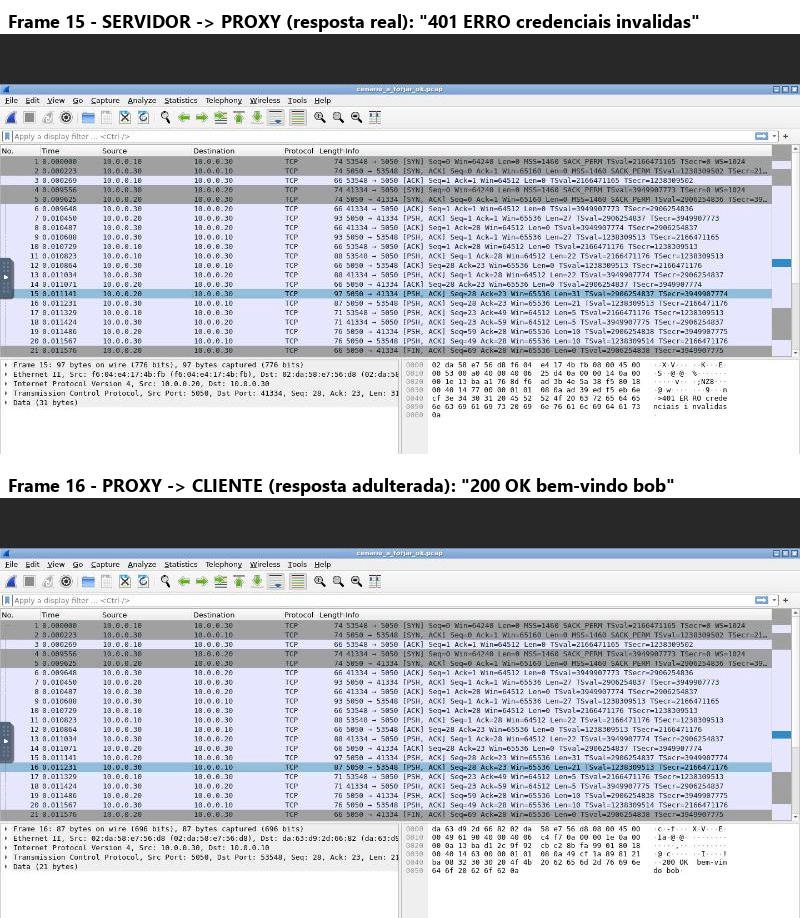
\includegraphics[width=\linewidth,keepaspectratio]{results/fase2/wireshark_mitm.png}
\caption{Wireshark: os dois fluxos TCP da mesma sessão divergem — o cliente
recebe \texttt{200 OK} enquanto o servidor enviou \texttt{401}.}
\label{fig:wireshark}
\end{figure}}{%
\textit{(Inserir aqui a captura \texttt{results/fase2/wireshark\_mitm.png} gerada
na demonstração ao vivo nas VMs do grupo.)}}

% =============================== 8. CONCLUSÃO ===============================
\section{Conclusão}

A Fase 2 cumpre seu objetivo: um proxy MITM, usando apenas sockets, posiciona-se
entre cliente e servidor, \textbf{lê e altera} as mensagens em trânsito e
\textbf{atende múltiplas sessões simultâneas} de forma robusta. Os três cenários
mostram que, sem integridade nem autenticação, uma resposta pode ser
\textbf{forjada} e um pedido pode ser \textbf{adulterado} — e o cliente/servidor
aceita a mensagem modificada \textbf{como legítima}, sem detecção.

Isso motiva diretamente a Fase 3: com \textbf{TLS} (confidencialidade +
integridade) e \textbf{autenticação do servidor por certificado}, o proxy não
conseguiria mais se passar pelo servidor nem alterar mensagens sem que a
validação do certificado/integridade acusasse a adulteração.

% =============================== APÊNDICES ===============================
\appendix
\newpage
\section{Instruções de execução (resumo)}
\label{ap:exec}

\begin{lstlisting}[style=saida]
# VM-servidor (inalterado, Fase 1)
python3 servidor.py --host 0.0.0.0 --porta 5050

# VM-atacante (proxy) -- iniciar ANTES do cliente
python3 proxy_mitm.py --escuta 0.0.0.0:5050 --servidor 10.0.0.20:5050 --forjar-ok

# VM-cliente (apontada ao PROXY, nao ao servidor)
python3 cliente.py --host 10.0.0.30 --porta 5050 --usuario bob --senha senhaERRADA

# Reproducao automatica em 3 namespaces (Linux, root)
sudo ./fase2/demo_mitm.sh
\end{lstlisting}

Detalhes completos (topologia, flags de adulteração, teste em \textit{loopback})
estão no \texttt{fase2/README.md}.

\newpage
\section{Código-fonte: \texttt{proxy\_mitm.py}}
\label{ap:codigo}
\lstinputlisting[language=Python]{../fase2/proxy_mitm.py}

\newpage
\section{Script de demonstração: \texttt{demo\_mitm.sh}}
\label{ap:demo}
\lstinputlisting[language=bash]{../fase2/demo_mitm.sh}

\newpage
\section{Log completo do proxy — concorrência e robustez}
\label{ap:concorrencia}
\lstinputlisting[style=saida]{results/fase2/D_concorrencia_proxy.txt}

\end{document}
